\documentclass[border=8pt]{standalone}
\usepackage[utf8]{inputenc}
\usepackage[T1]{fontenc}
\usepackage{lmodern}
\usepackage{amsmath}
\usepackage{siunitx}
\sisetup{output-decimal-marker={,}}
\usepackage{tikz}
\usetikzlibrary{
  arrows.meta,
  positioning,
  shapes.geometric,
  fit,
  backgrounds,
  calc,
  decorations.pathreplacing
}

% Report color palette (docs/relatorio/config/pacotes.tex)
\definecolor{wegblue}{RGB}{0, 87, 157}
\definecolor{slateink}{RGB}{38, 50, 56}
\definecolor{steelbg}{RGB}{244, 247, 250}
\definecolor{tealnode}{RGB}{0, 121, 107}
\definecolor{amberwarn}{RGB}{217, 119, 6}
\definecolor{crimsonalert}{RGB}{185, 28, 28}
\definecolor{ledgreen}{RGB}{22, 163, 74}
\definecolor{ledyellow}{RGB}{202, 138, 4}
\definecolor{ledred}{RGB}{220, 38, 38}
\definecolor{ledwhite}{RGB}{100, 116, 139}

\begin{document}
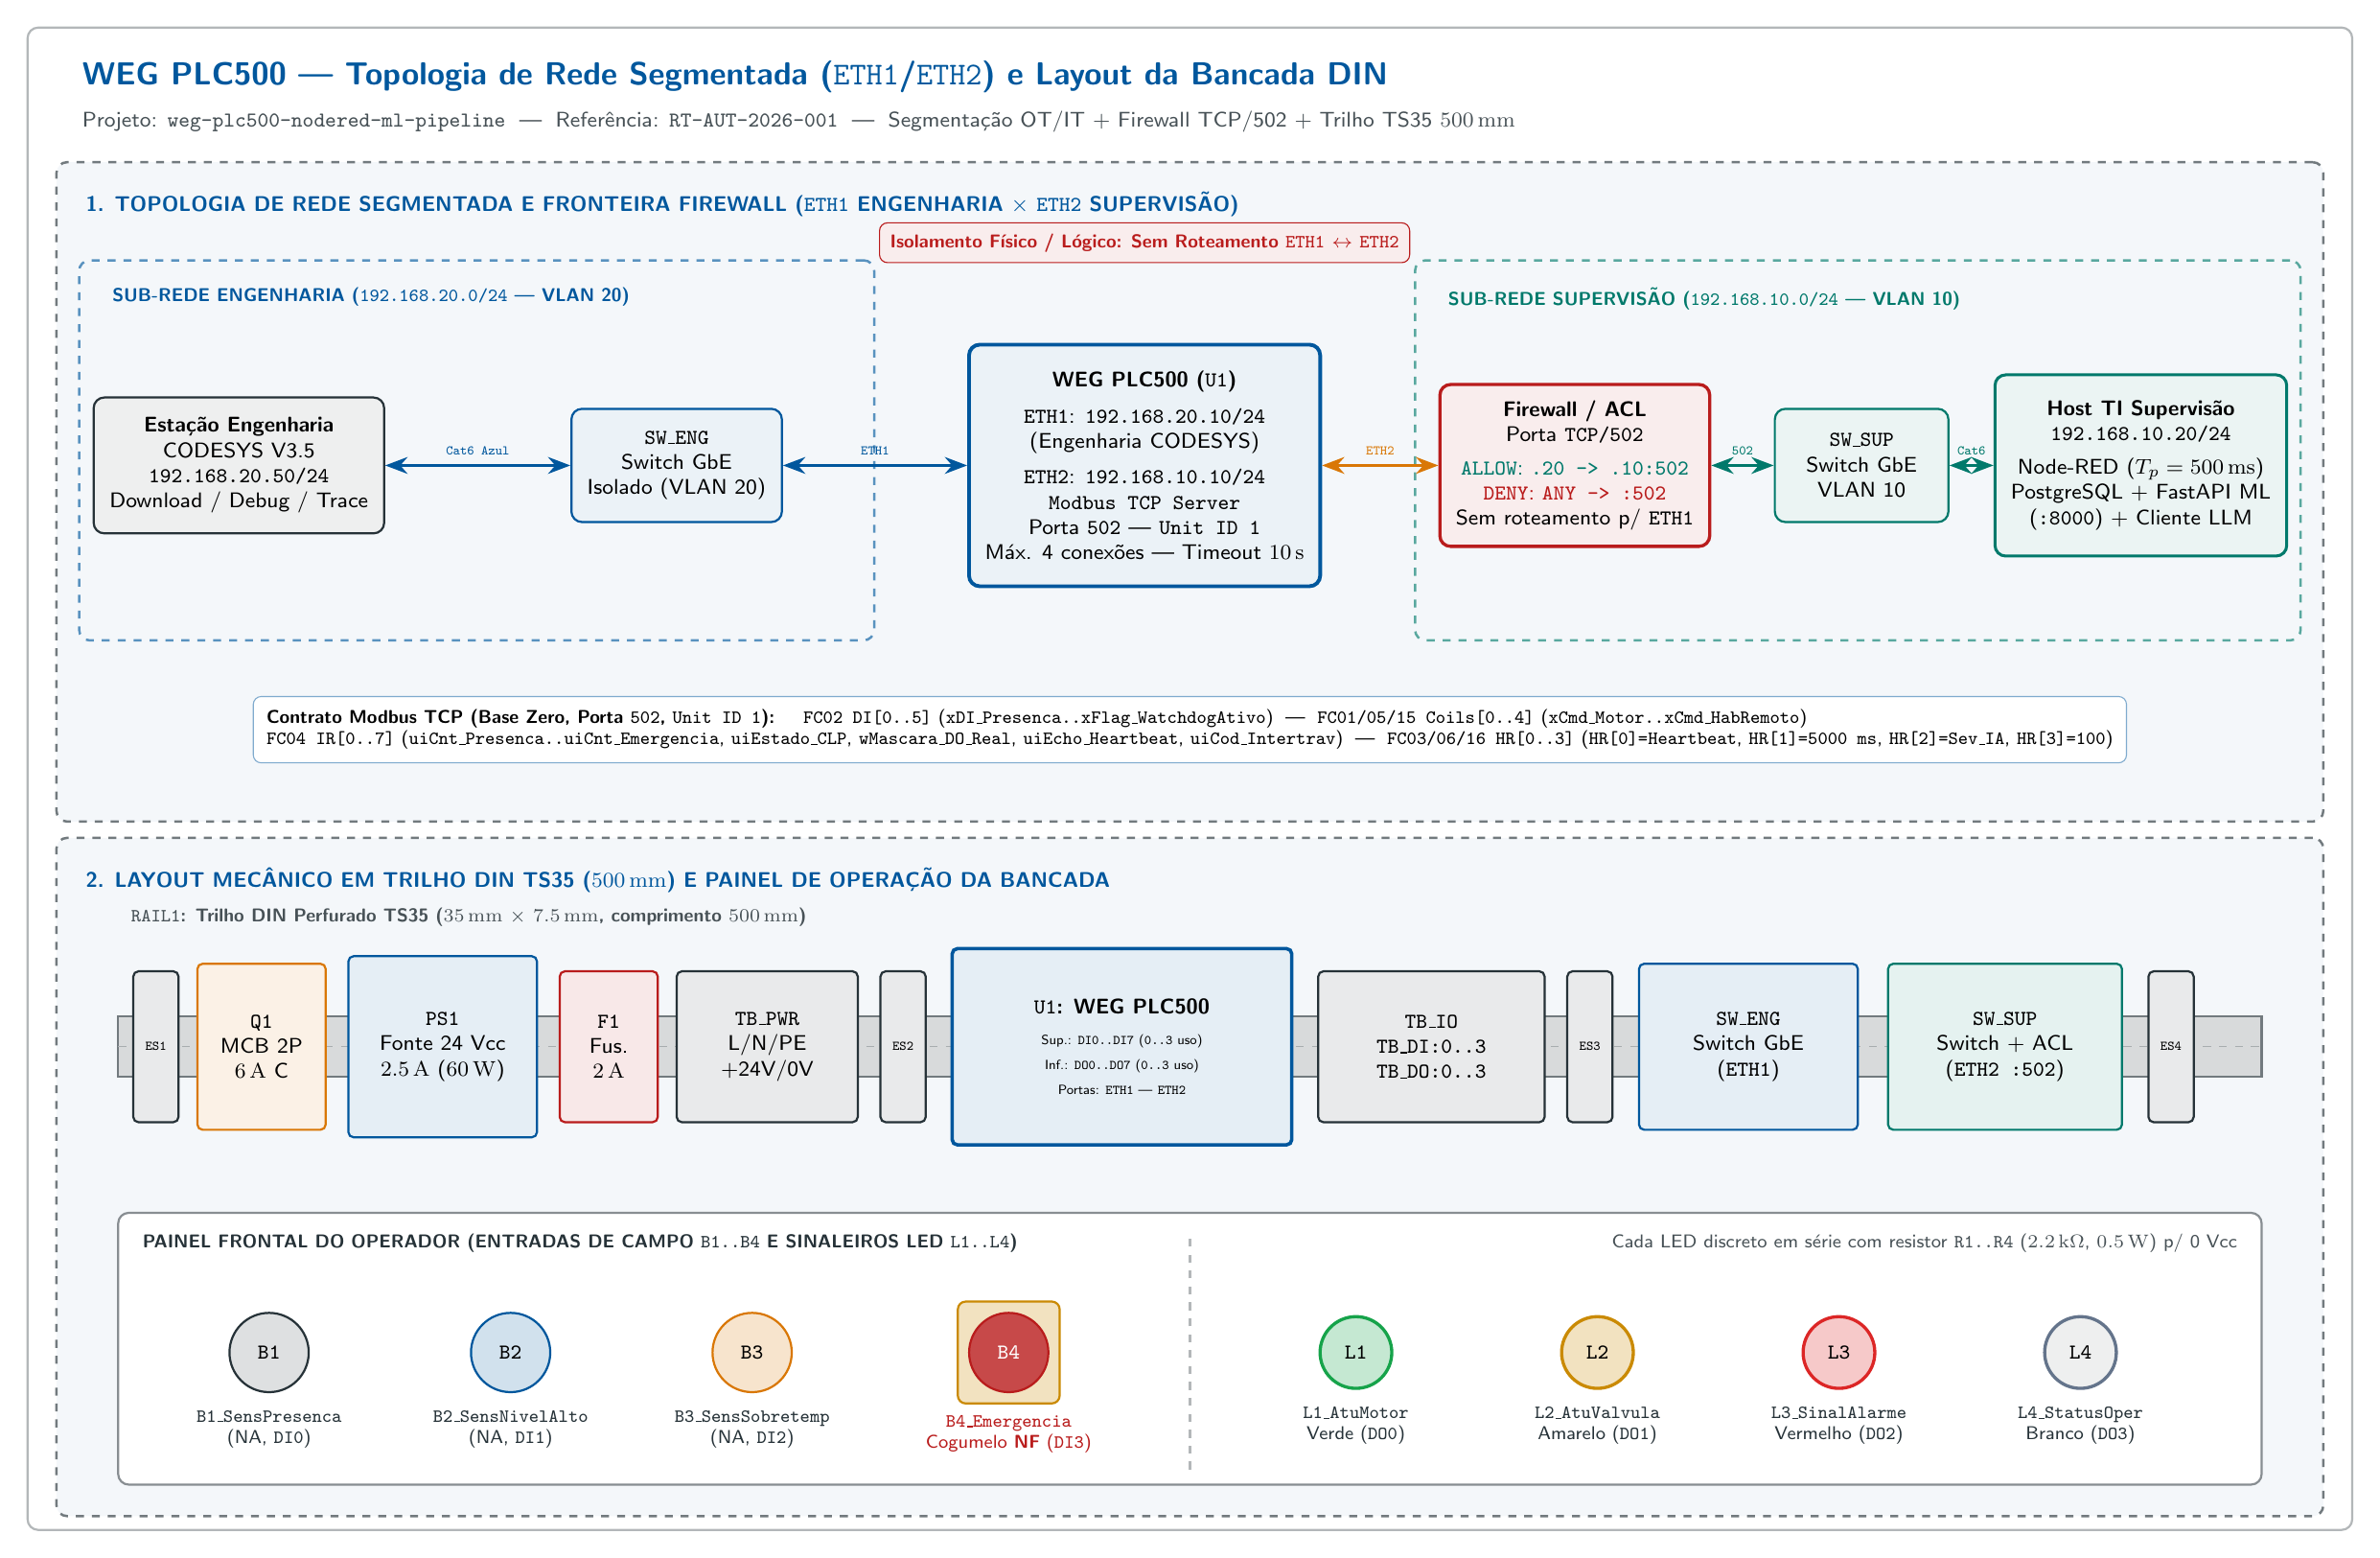
\begin{tikzpicture}[
  font=\sffamily\footnotesize,
  >=Stealth,
  netnode/.style={rectangle, rounded corners=4pt, draw=#1, fill=#1!8, thick, align=center, inner sep=6pt},
  zonebox/.style={rectangle, rounded corners=4pt, draw=#1!65, dashed, fill=steelbg, line width=0.9pt},
  dinmod/.style={rectangle, rounded corners=2pt, draw=#1, fill=#1!10, thick, align=center, inner sep=3pt},
  lbl/.style={font=\sffamily\scriptsize, text=slateink}
]

% =========================================================================
% OUTER FRAME & TITLE HEADER
% =========================================================================
\draw[draw=slateink!35, line width=0.8pt, rounded corners=4pt] (-0.4, 0.2) rectangle (30.4, 20.1);

\node[anchor=west, font=\sffamily\large\bfseries, text=wegblue] at (0.2, 19.45)
  {WEG PLC500 --- Topologia de Rede Segmentada (\texttt{ETH1}/\texttt{ETH2}) e Layout da Bancada DIN};
\node[anchor=west, font=\sffamily\footnotesize, text=slateink!85] at (0.2, 18.85)
  {Projeto: \texttt{weg-plc500-nodered-ml-pipeline} \;|\; Referência: \texttt{RT-AUT-2026-001} \;|\; Segmentação OT/IT + Firewall TCP/502 + Trilho TS35 \qty{500}{\milli\metre}};

% =========================================================================
% PANEL 1 (TOP): NETWORK SEGMENTATION & FIREWALL BOUNDARY
% =========================================================================
\begin{scope}[on background layer]
  \node[zonebox=slateink, fit={(0.1, 9.7) (29.9, 18.2)}] (panelNet) {};
  \node[zonebox=wegblue, fit={(0.4, 12.1) (10.7, 16.9)}] (zoneEng) {};
  \node[zonebox=tealnode, fit={(18.1, 12.1) (29.6, 16.9)}] (zoneSup) {};
\end{scope}

\node[anchor=north west, font=\sffamily\footnotesize\bfseries, text=wegblue] at (0.25, 18.05)
  {1. TOPOLOGIA DE REDE SEGMENTADA E FRONTEIRA FIREWALL (\texttt{ETH1} ENGENHARIA $\times$ \texttt{ETH2} SUPERVISÃO)};

\node[anchor=north west, font=\sffamily\scriptsize\bfseries, text=wegblue] at (0.6, 16.78)
  {SUB-REDE ENGENHARIA (\texttt{192.168.20.0/24} --- VLAN 20)};
\node[anchor=north west, font=\sffamily\scriptsize\bfseries, text=tealnode] at (18.3, 16.78)
  {SUB-REDE SUPERVISÃO (\texttt{192.168.10.0/24} --- VLAN 10)};

% Engineering Workstation
\node[netnode=slateink, minimum width=3.7cm, minimum height=1.8cm] (wsEng) at (2.4, 14.3)
  {\textbf{Estação Engenharia}\\CODESYS V3.5\\\texttt{192.168.20.50/24}\\Download / Debug / Trace};

% SW_ENG
\node[netnode=wegblue, minimum width=2.7cm, minimum height=1.5cm] (swEng) at (8.2, 14.3)
  {\textbf{\texttt{SW\_ENG}}\\Switch GbE\\Isolado (VLAN 20)};

% PLC500 Central Network Boundary (centered in clean gap between x=10.7 and x=18.1)
\node[netnode=wegblue, line width=1.4pt, minimum width=4.4cm, minimum height=3.2cm] (plcNet) at (14.4, 14.3)
  {\textbf{WEG PLC500 (\texttt{U1})}\\[4pt]
   \texttt{ETH1}: \texttt{192.168.20.10/24}\\
   (Engenharia CODESYS)\\[4pt]
   \texttt{ETH2}: \texttt{192.168.10.10/24}\\
   \texttt{Modbus TCP Server}\\
   Porta \texttt{502} | \texttt{Unit ID 1}\\
   Máx. 4 conexões | Timeout \qty{10}{\second}};

% Firewall ACL Box
\node[netnode=crimsonalert, line width=1.2pt, minimum width=3.4cm, minimum height=2.1cm] (fwBox) at (20.1, 14.3)
  {\textbf{Firewall / ACL}\\Porta \texttt{TCP/502}\\[3pt]
   \textcolor{tealnode}{\texttt{ALLOW}: \texttt{.20 -> .10:502}}\\
   \textcolor{crimsonalert}{\texttt{DENY}: \texttt{ANY -> :502}}\\
   Sem roteamento p/ \texttt{ETH1}};

% SW_SUP
\node[netnode=tealnode, minimum width=2.3cm, minimum height=1.5cm] (swSup) at (23.9, 14.3)
  {\textbf{\texttt{SW\_SUP}}\\Switch GbE\\VLAN 10};

% IT Host
\node[netnode=tealnode, line width=1.1pt, minimum width=3.6cm, minimum height=2.4cm] (itHost) at (27.6, 14.3)
  {\textbf{Host TI Supervisão}\\\texttt{192.168.10.20/24}\\[3pt]
   Node-RED ($T_p = \qty{500}{\milli\second}$)\\
   PostgreSQL + FastAPI ML\\
   (\texttt{:8000}) + Cliente LLM};

% Cat6 Ethernet Links
\draw[<->, very thick, wegblue] (wsEng.east) -- node[above, font=\sffamily\tiny]{\texttt{Cat6 Azul}} (swEng.west);
\draw[<->, very thick, wegblue] (swEng.east) -- node[above, font=\sffamily\tiny]{\texttt{ETH1}} (plcNet.west);

\draw[<->, very thick, amberwarn] (plcNet.east) -- node[above, font=\sffamily\tiny]{\texttt{ETH2}} (fwBox.west);
\draw[<->, very thick, tealnode] (fwBox.east) -- node[above, font=\sffamily\tiny]{\texttt{502}} (swSup.west);
\draw[<->, very thick, tealnode] (swSup.east) -- node[above, font=\sffamily\tiny]{\texttt{Cat6}} (itHost.west);

% Air-Gap / No Routing Callout cleanly positioned above PLC500 without touching zone headers
\node[draw=crimsonalert, fill=crimsonalert!8, rounded corners=3pt, font=\sffamily\scriptsize\bfseries, text=crimsonalert, inner sep=4pt] at (14.4, 17.25)
  {Isolamento Físico / Lógico: Sem Roteamento \texttt{ETH1} $\leftrightarrow$ \texttt{ETH2}};

% Modbus TCP Register Map Summary Box
\node[draw=wegblue!50, fill=white, rounded corners=3pt, inner sep=5pt, font=\sffamily\scriptsize, align=left] at (15.0, 10.8) {%
  \textbf{Contrato Modbus TCP (Base Zero, Porta \texttt{502}, \texttt{Unit ID 1}):} \quad
  \texttt{FC02 DI[0..5]} (\texttt{xDI\_Presenca..xFlag\_WatchdogAtivo}) \;|\;
  \texttt{FC01/05/15 Coils[0..4]} (\texttt{xCmd\_Motor..xCmd\_HabRemoto})\\
  \texttt{FC04 IR[0..7]} (\texttt{uiCnt\_Presenca..uiCnt\_Emergencia}, \texttt{uiEstado\_CLP}, \texttt{wMascara\_DO\_Real}, \texttt{uiEcho\_Heartbeat}, \texttt{uiCod\_Intertrav}) \;|\;
  \texttt{FC03/06/16 HR[0..3]} (\texttt{HR[0]=Heartbeat}, \texttt{HR[1]=5000 ms}, \texttt{HR[2]=Sev\_IA}, \texttt{HR[3]=100})
};

% =========================================================================
% PANEL 2 (BOTTOM): 35 mm TS35 DIN-RAIL & OPERATOR BENCH PANEL LAYOUT
% =========================================================================
\begin{scope}[on background layer]
  \node[zonebox=slateink, fit={(0.1, 0.5) (29.9, 9.25)}] (panelBench) {};
\end{scope}

\node[anchor=north west, font=\sffamily\footnotesize\bfseries, text=wegblue] at (0.25, 9.10)
  {2. LAYOUT MECÂNICO EM TRILHO DIN TS35 (\qty{500}{\milli\metre}) E PAINEL DE OPERAÇÃO DA BANCADA};

% Rail header cleanly above all DIN modules
\node[anchor=west, font=\sffamily\scriptsize\bfseries, text=slateink!85] at (0.85, 8.32)
  {\texttt{RAIL1}: Trilho DIN Perfurado TS35 (\qty{35}{\milli\metre} $\times$ \qty{7.5}{\milli\metre}, comprimento \qty{500}{\milli\metre})};

% TS35 DIN Rail metallic bar
\fill[slateink!18] (0.8, 6.2) rectangle (29.2, 7.0);
\draw[slateink!65, thick] (0.8, 6.2) rectangle (29.2, 7.0);
\draw[slateink!40, dashed] (0.8, 6.6) -- (29.2, 6.6);

% DIN Modules Left-to-Right
\node[dinmod=slateink, minimum width=0.6cm, minimum height=2.0cm] (es1) at (1.3, 6.6) {\tiny\texttt{ES1}};
\node[dinmod=amberwarn, minimum width=1.7cm, minimum height=2.2cm] (q1) at (2.7, 6.6) {\textbf{\texttt{Q1}}\\MCB 2P\\\qty{6}{\ampere} C};
\node[dinmod=wegblue, minimum width=2.5cm, minimum height=2.4cm] (ps1) at (5.1, 6.6) {\textbf{\texttt{PS1}}\\Fonte 24~Vcc\\\qty{2.5}{\ampere} (\qty{60}{\watt})};
\node[dinmod=crimsonalert, minimum width=1.3cm, minimum height=2.0cm] (f1) at (7.3, 6.6) {\textbf{\texttt{F1}}\\Fus.\\\qty{2}{\ampere}};
\node[dinmod=slateink, minimum width=2.4cm, minimum height=2.0cm] (tbpwr) at (9.4, 6.6) {\textbf{\texttt{TB\_PWR}}\\L/N/PE\\+24V/0V};
\node[dinmod=slateink, minimum width=0.6cm, minimum height=2.0cm] (es2) at (11.2, 6.6) {\tiny\texttt{ES2}};

\node[dinmod=wegblue, line width=1.3pt, minimum width=4.5cm, minimum height=2.6cm] (u1din) at (14.1, 6.6)
  {\textbf{\texttt{U1}: WEG PLC500}\\[2pt]
   \tiny Sup.: \texttt{DI0..DI7} (\texttt{0..3} uso)\\
   \tiny Inf.: \texttt{DO0..DO7} (\texttt{0..3} uso)\\
   \tiny Portas: \texttt{ETH1} | \texttt{ETH2}};

\node[dinmod=slateink, minimum width=3.0cm, minimum height=2.0cm] (tbio) at (18.2, 6.6) {\textbf{\texttt{TB\_IO}}\\\texttt{TB\_DI:0..3}\\\texttt{TB\_DO:0..3}};
\node[dinmod=slateink, minimum width=0.6cm, minimum height=2.0cm] (es3) at (20.3, 6.6) {\tiny\texttt{ES3}};
\node[dinmod=wegblue, minimum width=2.9cm, minimum height=2.2cm] (swengdin) at (22.4, 6.6) {\textbf{\texttt{SW\_ENG}}\\Switch GbE\\(\texttt{ETH1})};
\node[dinmod=tealnode, minimum width=3.1cm, minimum height=2.2cm] (swsupdin) at (25.8, 6.6) {\textbf{\texttt{SW\_SUP}}\\Switch + ACL\\(\texttt{ETH2 :502})};
\node[dinmod=slateink, minimum width=0.6cm, minimum height=2.0cm] (es4) at (28.0, 6.6) {\tiny\texttt{ES4}};

% =========================================================================
% OPERATOR BENCH PANEL STRIP (Bottom of Panel 2)
% =========================================================================
\draw[draw=slateink!55, fill=white, rounded corners=4pt, thick] (0.8, 0.8) rectangle (29.2, 4.4);
\node[anchor=north west, font=\sffamily\scriptsize\bfseries, text=slateink] at (1.0, 4.25)
  {PAINEL FRONTAL DO OPERADOR (ENTRADAS DE CAMPO \texttt{B1..B4} E SINALEIROS LED \texttt{L1..L4})};

% Pushbuttons B1..B4 (Left side)
\node[draw=slateink, fill=slateink!15, circle, minimum size=1.05cm, thick] (b1) at (2.8, 2.55) {\textbf{\texttt{B1}}};
\node[lbl, align=center, below=3pt of b1] {\texttt{B1\_SensPresenca}\\(NA, \texttt{DI0})};

\node[draw=wegblue, fill=wegblue!18, circle, minimum size=1.05cm, thick] (b2) at (6.0, 2.55) {\textbf{\texttt{B2}}};
\node[lbl, align=center, below=3pt of b2] {\texttt{B2\_SensNivelAlto}\\(NA, \texttt{DI1})};

\node[draw=amberwarn, fill=amberwarn!20, circle, minimum size=1.05cm, thick] (b3) at (9.2, 2.55) {\textbf{\texttt{B3}}};
\node[lbl, align=center, below=3pt of b3] {\texttt{B3\_SensSobretemp}\\(NA, \texttt{DI2})};

% B4 Mushroom E-stop on yellow collar
\node[draw=ledyellow, fill=ledyellow!25, rectangle, rounded corners=3pt, minimum size=1.35cm, thick] (b4base) at (12.6, 2.55) {};
\node[draw=crimsonalert, fill=crimsonalert!80, circle, minimum size=1.05cm, thick, text=white] (b4) at (12.6, 2.55) {\textbf{\texttt{B4}}};
\node[lbl, text=crimsonalert, align=center, below=5pt of b4] {\textbf{\texttt{B4\_Emergencia}}\\Cogumelo \textbf{NF} (\texttt{DI3})};

% Divider line between inputs and outputs
\draw[slateink!35, dashed, thick] (15.0, 1.0) -- (15.0, 4.1);

% Indicator LEDs L1..L4 (Right side)
\node[draw=ledgreen, fill=ledgreen!25, circle, minimum size=0.95cm, very thick] (l1) at (17.2, 2.55) {\textbf{\texttt{L1}}};
\node[lbl, align=center, below=3pt of l1] {\texttt{L1\_AtuMotor}\\Verde (\texttt{DO0})};

\node[draw=ledyellow, fill=ledyellow!25, circle, minimum size=0.95cm, very thick] (l2) at (20.4, 2.55) {\textbf{\texttt{L2}}};
\node[lbl, align=center, below=3pt of l2] {\texttt{L2\_AtuValvula}\\Amarelo (\texttt{DO1})};

\node[draw=ledred, fill=ledred!25, circle, minimum size=0.95cm, very thick] (l3) at (23.6, 2.55) {\textbf{\texttt{L3}}};
\node[lbl, align=center, below=3pt of l3] {\texttt{L3\_SinalAlarme}\\Vermelho (\texttt{DO2})};

\node[draw=ledwhite, fill=slateink!8, circle, minimum size=0.95cm, very thick] (l4) at (26.8, 2.55) {\textbf{\texttt{L4}}};
\node[lbl, align=center, below=3pt of l4] {\texttt{L4\_StatusOper}\\Branco (\texttt{DO3})};

\node[anchor=north east, font=\sffamily\scriptsize, text=slateink!85] at (29.0, 4.25)
  {Cada LED discreto em série com resistor \texttt{R1..R4} (\qty{2.2}{\kilo\ohm}, \qty{0.5}{\watt}) p/ 0~Vcc};

\end{tikzpicture}
\end{document}
